En este ejercicio mediremos la luz ambiente mostrándola por el display LCD y
enviándola por ordenador al mismo tiempo usando un fotorresistor. Este es el
montaje:

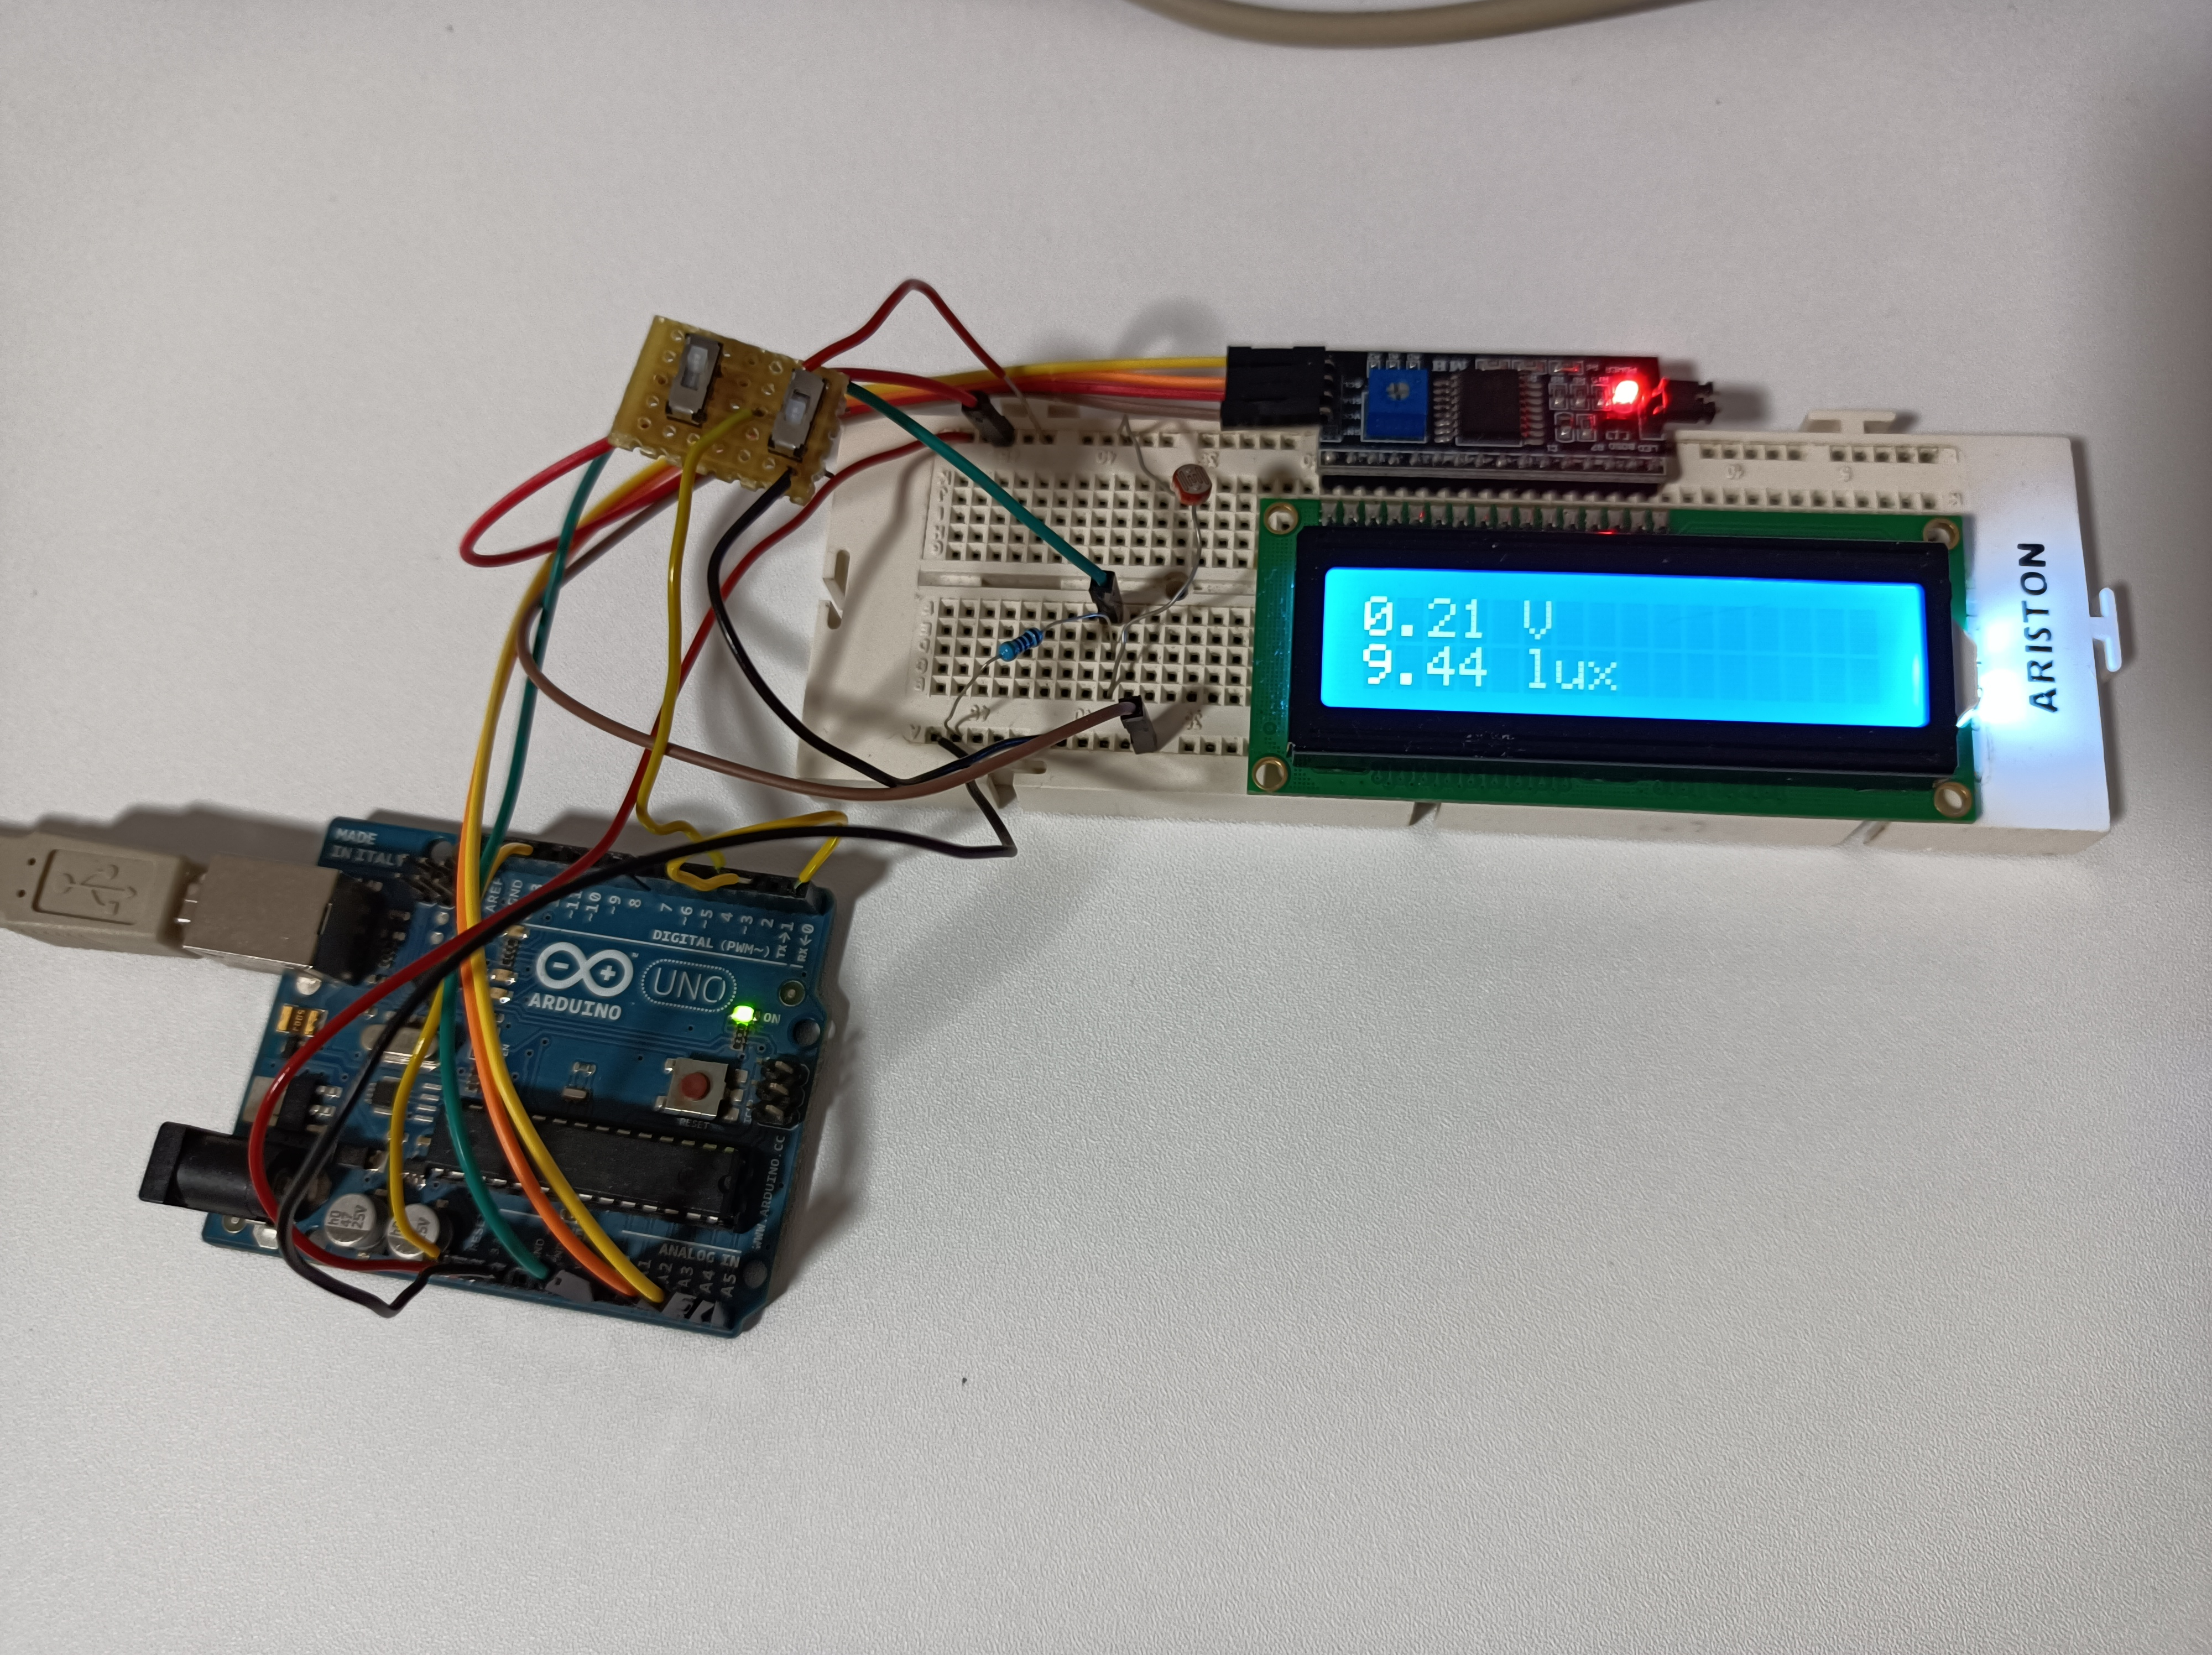
\includegraphics[width=\linewidth]{luxmeter-reader-wiring.jpg}

Para traducir las medidas de resistencia a cifras de luz (lux) con el
fotorresistor usado hay que aplicar la siguiente fórmula:

\begin{equation*}
L = 12518931 \cdot R_l^{-1.405}
\end{equation*}

Donde $L$ es el valor de luz en lux y $R_l$ es el valor de resistencia del
fotorresistor. Éste a su vez debe ser calculado de la siguiente manera:

\begin{gather*}
V_r = \frac{D}{D_{max}} \cdot V_{max} \\
V_l = V_{max} - V_r \\
R_l = \frac{V_l}{V_r} \cdot R_r
\end{gather*}

Donde $D$ es la lectura de valor analógico entre la resistencia y el
fotorresistor, $V_{max}$ la tensión máxima que soporta el pin analógico (que en
este caso son \emph{5 V}), $D_{max}$ la lectura máxima que puede devolver el
puerto (que en este caso es \emph{1023}), $V_r$ es la caída de tensión entre
los terminales de la resistencia, $V_l$ la caída de tensión entre los
terminales del fotorresistor, $R_r$ es el valor de la resistencia fija
(\emph{1 K$\Omega$}) y $R_l$ el valor de resistencia del fotorresistor.

La programación de la placa Arduino se realizaría así teniendo en cuenta estos
procedimientos:

\lstinputlisting[language=C++, caption=luxmeter-reader.ino]{
    1/luxmeter-reader/luxmeter-reader.ino
}

Para la aplicación cliente en el ordenador, creamos un proyecto llamado
\verb|luxmeter-reader| que recibirá las lecturas.

\lstinputlisting[caption=luxmeter-reader/Cargo.toml]{
    1/luxmeter-reader/Cargo.toml
}

\lstinputlisting[language=Rust, caption=luxmeter-reader/src/main.rs]{
    1/luxmeter-reader/src/main.rs
}